\documentclass[conference]{IPEC2026}
\IEEEoverridecommandlockouts
% The preceding line is only needed to identify funding in the first footnote. If that is unneeded, please comment it out.
%Template version as of 6/27/2024

\usepackage{cite}
\usepackage{amsmath,amssymb,amsfonts}
\usepackage{algorithmic}
\usepackage{graphicx}
\usepackage{textcomp}
\usepackage{xcolor}
\def\BibTeX{{\rm B\kern-.05em{\sc i\kern-.025em b}\kern-.08em
    T\kern-.1667em\lower.7ex\hbox{E}\kern-.125emX}}
\begin{document}

\title{Holistic Efficiency Optimization of Traction Drives Accounting for Machine Harmonic Losses using an Improved Impedance-based Modelling
% : Analysis and Mitigation Strategies
\\
% {\footnotesize \textsuperscript{*}Note: Sub-titles are not captured in Xplore and
% should not be used}
\thanks{Research leading to these results has received funding from the EU CHIPSJoint Undertaking under grant agreement $n^o$ 101007326 (project PowerizeD) and from the (Swedish) partner national funding authority Vinnova. Funding for this research has also been received from the Swedish Energy Agency under grant agreement P2022-00956 through the HEMIZERO project.
%by the Chips Joint Undertaking
}
}

% Please replace * with your track number
\track{: 6 Vehicle Electrification-related Technologies}


\maketitle

\begin{abstract}
The electrification of heavy-duty vehicles is crucial for reducing greenhouse gas emissions and achieving sustainable transportation. High-efficiency traction systems, including inverters and machines, play a central role in this transition. 
Although the loss analysis for the inverter side is well-studied, harmonic loss of the motor side is still worth investigating, and traditional optimization approaches treat these components independently, resulting in suboptimal system efficiency.
This study highlights the trade-off between motor and inverter losses, driven by switching frequency, and emphasizes the need for a holistic system-level perspective. 
Further, a new loss factor modeling approach is proposed to estimate motor harmonic losses accurately, optimizing total system efficiency while maintaining sustainability.
\end{abstract}

\begin{IEEEkeywords}
component, formatting, style, styling, insert.
\end{IEEEkeywords}

\section{Introduction}

The electrification of heavy-duty vehicles is one of the milestones to reach sustainable transportation, providing significant reductions in greenhouse gas emissions compared to combustion engine rivals \cite{ElectrificationVehicles}. 
At the heart of this transition lies the development of high-efficiency traction systems, comprising the inverter and electric machine, which are critical for minimizing energy losses and achieving sustainability goals \cite{HeartOfTraction,Outlook_EV}.
Traditional optimization methods to achieve a high-efficiency traction system often treat inverters and machines as independent entities, neglecting their interactions \cite{Traditional_Optimization,Traditional_Optimization_2}. 
However, the non-sinusoidal current waveforms produced by pulse-width modulation (PWM) inverters result in additional machine losses, called harmonic losses \cite{PWMLoss1,PWMLoss3}. 
Therefore, a critical challenge in achieving optimal system efficiency lies in balancing the trade-off between PWM-related motor harmonic losses and inverter losses \cite{PWMLoss2}. 
For instance, as switching frequency increases, inverter losses rise due to higher switching events, while motor harmonic losses decrease as the current ripple diminishes and harmonics shift to higher frequencies. 
Inverter efficiency modeling and optimization have been extensively explored in the literature, focusing on parameters such as switching frequency and die area \cite{DieAreaOptimization}. 
However, accurate estimation of motor harmonic losses remains a challenging task and is worth investigating deeply. 

Studies have investigated the impact of PWM inverter on machine losses, considering factors like: switching frequency and modulation strategies \cite{PWM_motor_studies, PWM_motor_studies2}.
Estimating PWM-induced machine losses can be approached through both modeling/simulation and experimental methods, each offering unique advantages and challenges.
The modeling/simulation approach, often utilizing finite element analysis (FEA), provides detailed insights into losses within windings and stator/rotor cores \cite{Modelling_PWM_loss, Modelling_PWM_loss_2,Modelling_PWM_loss_3}.
While this method can accurately capture the spatial distribution of losses, it is computationally expensive and may be less precise when the losses are a small fraction of the transferred power.
On the other hand, the experimental approach involves techniques like harmonic injection and impedance measurement, which isolate specific harmonic losses and loss separation between fundamental and harmonic components, helping to distinguish the impact of high-frequency switching \cite{Impedance_based,harmonic_injection, Harmonic_injection_2}. 
The main idea in these methods is to extract a loss factor regarding each frequency component, which, later on, might be implemented into the optimization to calculate the losses for specific modulations. In these methods, frequency-domain superposition is regarded, and the power losses are estimated independently for different frequency components.  
%find a sweet operating point of switching frequency for specific modulations.
However, it is experimentally observed that the dynamic behavior of motors often results in interaction between harmonics, which causes discrepancies. 

%persistent discrepancies, underscoring the need for more precision.

In the literature, the interaction of the harmonics, which affects the loss factor of the experimental modeling, has not been studied well. 
The interaction is investigated for induction machines in \cite{interaction_harmonics} and for rotor losses in \cite{rotor_losses_1,rotor_losses_2}, but it is still not clear how to implement the modulated waveforms into the loss factor calculation to estimate the harmonic losses at specific operating points of the traction drive. 
This study proposes a method to add the effect of pair harmonics into impedance-based loss modelling to improve the estimation of motor harmonic losses, enabling a more accurate and integrated evaluation of total system efficiency. 
Then, a holistic approach to efficiency optimization is proposed to find the optimum switching frequency and die area of the selected power switches. 

% This paper is organized as follows. 
% Section II provides system specifications and requirements 
% Section III provides system specifications and requirements 
% Section IV provides system specifications and requirements 
% Section V provides system specifications and requirements 


\section{System Specifications and Requirements}
Beyond efficiency, reducing the component count —such as minimizing the number of semiconductors, isolated gate drivers, and control resources —contributes to a smaller carbon footprint and promotes the development of more sustainable systems.
%In this context, two-level three-phase drives remain a viable solution.
Compared to multi-level and multi-phase systems, two-level and three-phase configurations require fewer components, which simplifies system design and reduces complexity while maintaining operational efficiency. 
These advantages still make two-level three-phase systems an attractive choice for heavy-duty vehicle applications, where reliability, cost-effectiveness, and sustainability are paramount.
Table \ref{tab:systempar} outlines the system specifications for heavy-duty vehicles in the current application.
To ensure efficient and reliable megawatt charging, a DC-link voltage of 1250V has been selected.
The system's power rating, determined as 300kW, is based on the vehicle dynamics and the load requirements of heavy-duty vehicles.
The traction system utilizes a 3-phase configuration, with phase voltage and current designed to meet the specified power rating.
The optimal switching frequency, within the range of 10kHz to 30kHz, is chosen based on the power devices and system requirements.

\begin{table}[h]
\centering
\caption{System Specifications and Requirements}
\begin{tabular}{ll}
\textbf{Parameter }& Value \\
\hline
\hline
\textbf{Power Rating}& $300~kW$ \\
\textbf{Input Voltage $\mathrm{V_{in}}$} & $1250~V$ \\
\textbf{Input Current $\mathrm{I_{in}}$} & $240~A$ \\
\textbf{Phase Voltage $\mathrm{V_{pn}}$} & $625~V$ \\
\textbf{Power Factor $\mathrm{p_{f}}$} & $0.9$ \\
\textbf{Phase Current $\mathrm{I_{p}}$} & $356~A$\\
\textbf{Switching Frequency $\mathrm{f_{s}}$} & $10-30~kHz$ \\
\hline 
\\
\end{tabular}
\label{tab:systempar}
\end{table}


\section{Motor Harmonic Loss Estimation: Improved Impedance Model}

\subsection{Conventional Frequency-Domain Method}

A common approach models the machine by a frequency-dependent impedance $Z(j\omega)$, obtained via LCR measurement or harmonic injection, as shown in Fig.~\ref{fig:impedance_motor}.  
From this, a voltage-based \emph{loss factor} is extracted:
\begin{equation}
    \Phi(\omega) = \frac{P_{\text{add}}(\omega)}{|V(\omega)|^2},
    \label{eq:loss_factor}
\end{equation}
where $P_{\text{add}}(\omega)$ is the additional loss caused by a voltage component $V(\omega)$.  
The harmonic losses are then computed by superposition:
\begin{equation}
    P_{\text{harm}} = \sum_{n\neq 1} \Phi(\omega_n)\,|V_n|^2,
    \label{eq:freq_loss}
\end{equation}
with $\omega_n = n\omega_e$.  
This method assumes negligible saturation and saliency ($L_d \!\approx\! L_q$).

\begin{figure}[h!]
    \centering
    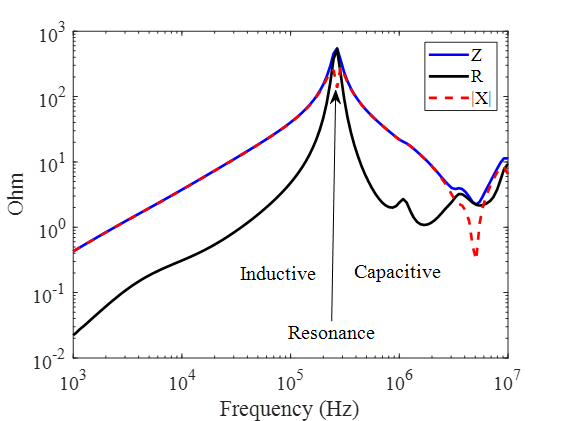
\includegraphics[width=0.7\linewidth]{Figures/HarmonicLoss/ImpadanceMotor.png}
    \caption{Impedance measurement of the machine.}
    \label{fig:impedance_motor}
\end{figure}

\subsection{Effect Saliency and Saturation}

Experimental waveforms under inverter excitation (Fig.~\ref{fig:voltagecurrentTime}) reveal that the FFT-based power spectrum (Fig.~\ref{fig:powerFFT}) contains negative components, i.e., some harmonics appear as generating power.  
This indicates interaction between harmonics, which the independent-harmonic model cannot explain.

\begin{figure}[h!]
    \centering
    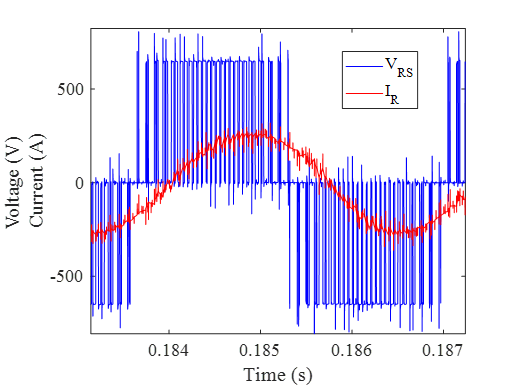
\includegraphics[width=0.7\linewidth]{Figures/HarmonicLoss/voltageCurrentTime.png}
    \caption{Measured phase voltage and current.}
    \label{fig:voltagecurrentTime}
\end{figure}

\begin{figure}[h!]
    \centering
    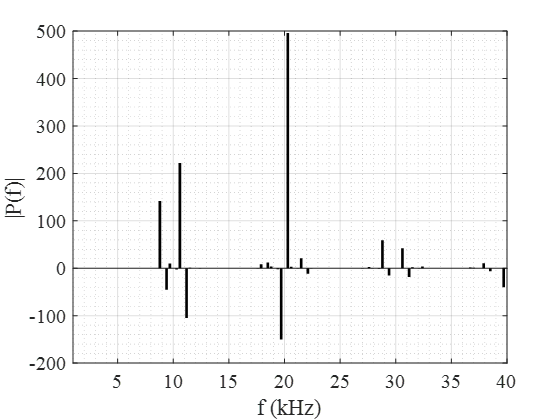
\includegraphics[width=0.7\linewidth]{Figures/HarmonicLoss/FFTPower_exp.png}
    \caption{Measured harmonic power spectrum.}
    \label{fig:powerFFT}
\end{figure}

The effect originates from saliency ($L_d \neq L_q$), which modulates the inductance at $2\omega_e$:
\begin{equation}
    L(t) = L_0 + \Delta L \,\sin(2\omega_e t - \theta),
    \label{eq:L_time}
\end{equation}
with $L_0=(L_d+L_q)/2$, $\Delta L=(L_q-L_d)/2$. In the frequency domain, this creates cross-admittances $Y_{n,m}$ that couple harmonics separated by two indices:
\begin{equation}
    I_n \approx Y_n V_n + \sum_m Y_{n,m}V_m, \quad Y_{n,m}\neq0 \;\; \text{if}\; |n-m|=2.
    \label{eq:mixing}
\end{equation}

\subsection{Extended Formulation with Harmonic Pair Interaction in Stator}

To capture these effects, the loss model is extended with cross terms:
\begin{equation}
    P_{\text{harm}} = \sum_{n\neq 1} \Phi_s(\omega_n)\,|V_n|^2
    + \sum_{\substack{n\neq m \\ |n-m|=2}} \chi_{n,m}\,\Re\{V_n V_m^{*}\},
    \label{eq:saliency_loss}
\end{equation}
where $\Phi_s(\omega)$ is the stator loss factor and $\chi_{n,m}$ are interaction coefficients identified experimentally.  
Negative spectral bars arise when $\Re\{V_n V_m^{*}\}<0$ or $\chi_{n,m}<0$, reflecting partial cancellation.

\subsection{Harmonic Interaction in Rotor Losses}
Rotor losses are also subject to harmonic interaction. After the $2\omega_e$ modulation, each current harmonic can be decomposed into positive and negative sequences:
\begin{align}
    I_{+,n} =& \tfrac{1}{3}(I_{a,n}+a^2 I_{b,n}+a I_{c,n}), \\
    I_{-,n} =& \tfrac{1}{3}(I_{a,n}+a I_{b,n}+a^2 I_{c,n}),
    \label{eq:seq_decomp}
\end{align} 

with $a=e^{j2\pi/3}$.  Because the rotor rotation shifts the apparent frequency differently—positive-sequence components appear at a reduced frequency and negative-sequence components at an increased frequency—certain positive–negative sequence pairs align to the same rotor frequency and thus interact.  
% The generalized formulation distinguishes stator and rotor contributions for both sequences:
% \begin{equation}
% \begin{aligned}
%     P_{\text{harm}} = \sum_{n\neq 1} &\Big(
%     \Phi_{s}^{(+)}(\omega_{r,n}^{(+)}) |V_{+,n}|^2 +
%     \Phi_{r}^{(+)}(\omega_{r,n}^{(+)}) |V_{+,n}|^2 \\
%     &+
%     \Phi_{s}^{(-)}(\omega_{r,n}^{(-)}) |V_{-,n}|^2 +
%     \Phi_{r}^{(-)}(\omega_{r,n}^{(-)}) |V_{-,n}|^2
%     \Big),
% \end{aligned}
% \label{eq:seq_loss}
% \end{equation}
% where $\Phi_{s}^{(\pm)}$ and $\Phi_{r}^{(\pm)}$ are the stator and rotor loss factors, and $\omega_{r,n}^{(\pm)}$ are the rotor frequencies seen by each sequence.  
In the present machine, however, these rotor harmonics losses are much smaller than the stator harmonic losses. For modelling feasibility, rotor terms are therefore neglected, and only the dominant stator harmonic interactions are explicitly considered.



% \section{Inverter Loss Modelling}

% The total inverter losses comprise conduction and switching losses.  
% For a single MOSFET, the conduction loss is
% \begin{equation}
%     \label{eq:conductionlosses}
%      P_c = \frac{1}{2\pi} \int_{\theta_{C1}}^{\theta_{C2}} r_{ds} \, i_{ds}^2(\theta) D(\theta)\,d\theta ,
% \end{equation}
% where $r_{ds}$ is the on-state resistance, $i_{ds}(\theta)$ the device current, $D(\theta)$ the duty ratio, and $\theta_{C1}$–$\theta_{C2}$ the conduction interval.  
% Body diode conduction is neglected, which slightly overestimates reverse conduction and underestimates dead-time losses, partly compensating each other \cite{PotentialAircraft}.

% Switching losses consist of zero-current energy and overlap energy \cite{FOMSiC}.  
% The former depends on device output capacitance,
% \begin{equation}
% \label{eq:Psw-0}
%      E_{sw,ZCS} = C_{oss,Q}(U_{dc}) \, U_{dc}^{2},
% \end{equation}
% while the latter depends on current and voltage slopes,
% \begin{equation}
% \label{eq:overlapped}
%      \begin{split}
%      E_{sw,ov} &= \frac{V_{dc} I_{sw}^2}{2\, \tfrac{di}{dt_{on}}} + \frac{V_{dc}^2 I_{sw}}{2\, \tfrac{dv}{dt_{on}}} \\
%      &+ \frac{V_{dc} I_{sw}^2}{2\, \tfrac{di}{dt_{off}}} + \frac{V_{dc}^2 I_{sw}}{2\, \tfrac{dv}{dt_{off}}}.
%     \end{split}
% \end{equation}
% Total switching losses are then
% \begin{equation}
%     \label{eq:switching_general}
%      P_{sw} = \frac{f_{sw}}{2\pi} \int_{\theta_{SW1}}^{\theta_{SW2}} (E_{sw,ov} + E_{sw,ZCS}) \, d\theta .
% \end{equation}


% \subsection{Semiconductor Loss Modelling}

% The inverter losses are divided into two main parts: conduction and switching losses of the semiconductor. 
% The conduction loss for a single switch can be calculated as given by 
% \begin{equation}
%     \label{eq:conductionlosses}
%      P_c = \frac{1}{2\pi} \int_{\theta_{C1}}^{\theta_{C2}} r_{ds} \cdot i_{ds}(\theta)^2 \cdot D(\theta)\,d\theta 
% \end{equation}
% where duty cycles ($ D(\theta)$), switch current ($i_{ds}(\theta)$), conduction angles ($ \theta_{C1}$ to $\theta_{C2}$), and on-state resistance ($r_{ds}$) are required.
% While calculating conduction losses, the effect of the body diode can be ignored in the reverse conduction of MOSFETs and during dead times. 
% Ignoring the body diode leads to overestimating the loss during the reverse conduction and underestimating the loss during the dead times \cite{PotentialAircraft}. 
% Therefore, these assumptions partly compensate for each other. 

% The switching loss comprises two main components: zero current switching loss and overlapping loss \cite{FOMSiC}. 
% The zero current switching energy is reliant on the output capacitance ($C_{oss,Q}$) and switching voltage ($U_{dc}$); however, the overlapping energy is proportionate to $ \dfrac{dV}{dt}$ and $ \dfrac{di}{dt}$.
% Firstly, the zero current switching energy can be estimated as given by 
% \begin{equation}
% \label{eq:Psw-0}
%      \begin{split}
%      E_{sw-ZCS} &=C_{oss,Q}(U_{dc}) \cdot U_{dc}^{2} 
%     \end{split}
% \end{equation}
% Secondly, the overlapping switching energy can be calculated as given by 
% \begin{equation}
% \label{eq:overlapped}
%      \begin{split}
%      E_{sw-overlapping} &= (\dfrac{V_{dc} \cdot I_{sw}^2}{2 \cdot\frac{di}{dt_{on}}} +  \dfrac{V_{dc}^2 \cdot I_{sw}}{2 \cdot\frac{dv}{dt_{on}}})  \\
%      &+ (\dfrac{V_{dc} \cdot I_{sw}^2}{2 \cdot\frac{di}{dt_{off}}} +  \dfrac{V_{dc}^2 \cdot I_{sw}}{2 \cdot\frac{dv}{dt_{off}}})
%     \end{split}
% \end{equation}
% where  $ \dfrac{dV}{dt}$ and $ \dfrac{di}{dt}$ should be selected regarding layout parasitics, gate driver and isolation requirements of the motor. 
% Finally, the total switching losses can be calculated by using 
% \begin{equation}
%     \label{eq:switching_general}
%      P_{sw} = \frac{f_{sw}}{2\pi} \int_{\theta_{SW1}}^{\theta_{SW2}}   (E_{sw-overlapping}(\theta)+ E_{sw-ZCS}(\theta))\,d\theta 
% \end{equation}
% during a switching angle ($\theta_{SW1}$ to $\theta_{SW2}$). 


% \subsection{2-Level Inverter Loss Modelling }

% The conduction and switching angles for switches and diodes are employed in calculating the semiconductor losses using (\ref{eq:conductionlosses}), (\ref{eq:switching_general}).


% As presented in Table \ref{tab:2L_cond}, the angles for each switch in a single leg during a positive half-cycle of the line current can be provided. 
% It is also necessary to recognize that the switching voltage equals the DC-link voltage.

% \begin{table}[h]
% \centering
% \caption{Conduction and Switching Angles for 2L-3Ph  \cite{PotentialAircraft}.}
% \begin{tabular}{ccccc}

% \textbf{Switch} & \textbf{Conduction Angle}  & \textbf{Duty ratio}  & \textbf{Switching Angle} \\
% % & ($\gamma_1$ to $\gamma_2$) & ($D(\gamma)$) & ($\gamma_3$ to $\gamma_4$) \\
% \hline  \hline 
% Upper &  $\phi$ to $\pi + \phi $ & $\frac{1 + m_a\cdot sin(\theta)}{2} $&  $\phi$ to $\pi + \phi $ \\ \hline
% Lower* &  $\phi$ to $\pi + \phi $  & $\frac{1 - m_a\cdot sin(\theta)}{2} $ &  - \\
% \hline \hline 
% % Upper* &   $\pi + \phi $ to $2\pi + \phi $ & $\frac{1 - m_a\cdot sin(\theta)}{2} $&  -\\ \hline
% % Lower &  $\pi + \phi $ to $2\pi + \phi $ & $\frac{1 - m_a\cdot sin(\theta)}{2} $ & $\pi + \phi $ to $2\pi + \phi $ \\
% % \hline 
% % \hline 
% \end{tabular}
% % \begin{tablenotes}
% %       \scriptsize
% %       \item * means that the switch is in reverse conduction.
% % \end{tablenotes}
% \label{tab:2L_cond}
% \end{table}


\section{Holistic Efficiency Optimization of the Traction System}

\subsection{The Selection of Power Switch and Inverter Loss Map}
Selecting the voltage rating of a switch has a noteworthy impact on the design stage of the traction inverter. 
It is often selected higher than the blocking voltage with a safety factor to account for voltage overshoots caused by high switching speeds and layout parasitics, and the effect of cosmic rays on reliability \cite{layout2}.
In our system, the safety factor of 1.6 is selected, leading to the switches' voltage ratings of 2000 V for 2-level topologies. 
Furthermore, the current rating of the switch plays a critical role in the efficiency performance of the inverter. 

\begin{figure}[h!]
    \centering
    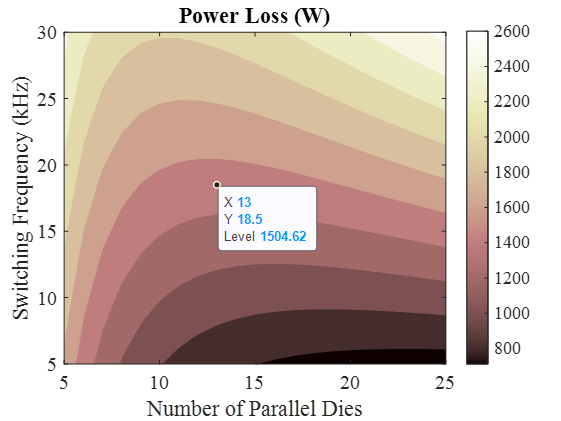
\includegraphics[width=0.7\linewidth]{Figures/HolisticOptimization/DieAreaSwitchingFrequency.png}
    \caption{Inverter losses map for varying switching frequency and die-area.}
    \label{fig:powerFFT}
\end{figure}


\begin{figure}[h!]
    \centering
    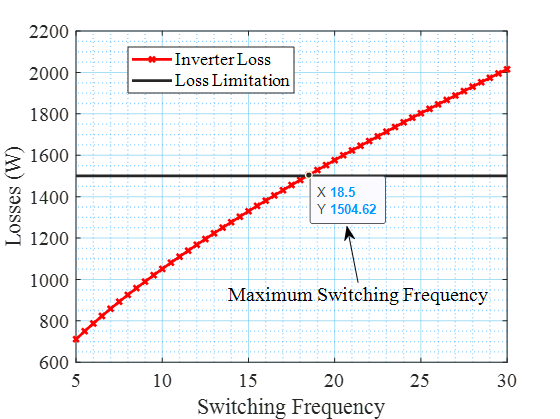
\includegraphics[width=0.7\linewidth]{Figures/HolisticOptimization/MaxSwitchingOnlyInverter.png}
    \caption{Power losses versus switching frequency for the optimized die area. }
    \label{fig:powerFFT}
\end{figure}

\subsection{The Loss Factor Of The Machine}

\begin{figure}[h!]
    \centering
    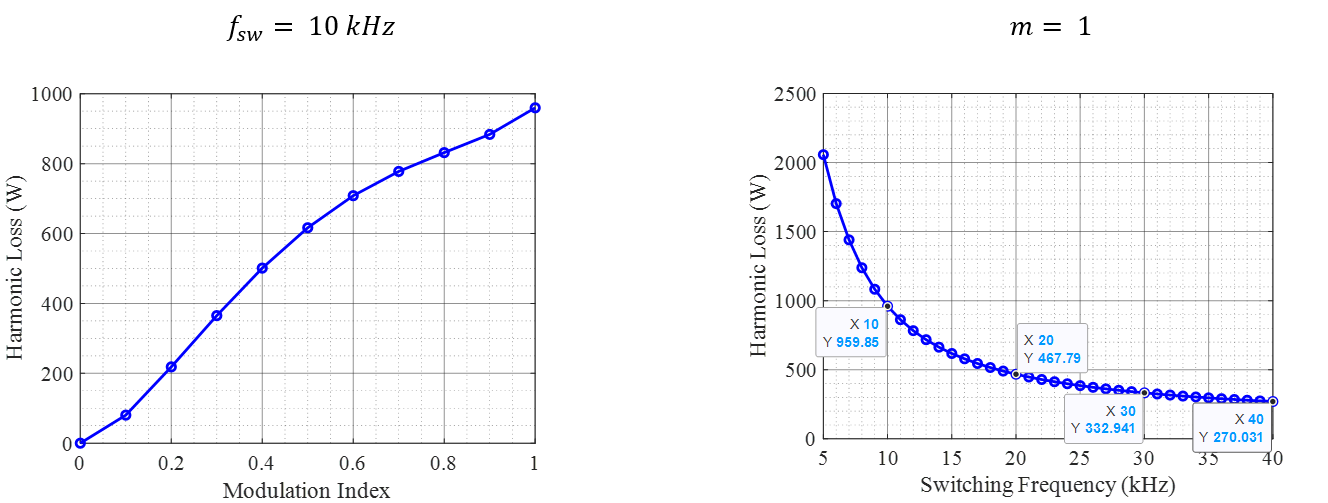
\includegraphics[width=1\linewidth]{Figures/HolisticOptimization/MotorHarmonicLosses.png}
    \caption{Motor Harmonic Losses.}
    \label{fig:powerFFT}
\end{figure}


\subsection{Loss Trade-off}
\begin{figure}[h!]
    \centering
    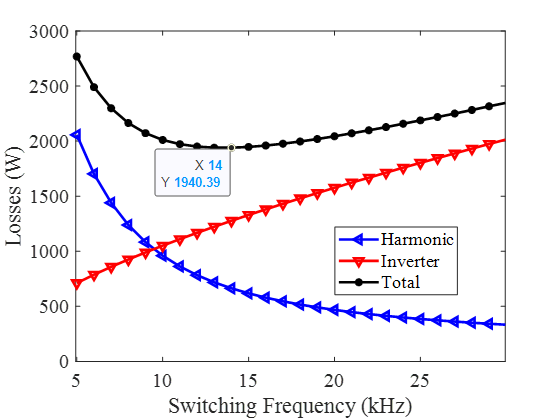
\includegraphics[width=0.7\linewidth]{Figures/HolisticOptimization/OverallLossOptimization.png}
    \caption{Overall Loss Optimization}
    \label{fig:powerFFT}
\end{figure}


\color{red}
The remaining parts will be given in the full paper.

\section{Experimental Validation}

\section{Conclusion }


\color{black}
\bibliographystyle{IEEEtran}
%\vspace*{-4mm}
\bibliography{ref.bib}


\end{document}
